
\chapter{Classical definitions of energy flux in solids}  \label{ch:appendix-carbogno}

In this appendix we demonstrate the equivalence between two formulations of the classical energy current in solids, Eqs.~\eqref{eq:J-classical} and \eqref{eq:J-leyla}, by using the gauge invariance principle presented in Sec.~\ref{sec:gauge-invariance}. 

Let us consider the general formula of the energy flux for classical force fields, Eq.~\eqref{eq:J-classical}, and rewrite it in the following way:
\begin{align}
    \mathbf{J}_A^\smallE (\rGamma) &= \frac{1}{\Omega} \sum_n \left( \mathbf{J}_c^\smallE + \mathbf{J}_v^\smallE \right) \nonumber\\
        &= \frac{1}{\Omega} \sum_n \left( \dot{\mathbf{R}}_n \epsilon_n + \mathbf{R}_n \dot{\epsilon}_n \right) , \label{eq:apx-J-classical}
\end{align}
where $\mathbf{J}_c^\smallE$ and $\mathbf{J}_v^\smallE$ are the ``convective'' and ``virial'' components of the energy flux, as defined in Eqs.~(\ref{eq:J-convective}-\ref{eq:J-virial}). 
In solids, the definition of Eq.~\eqref{eq:J-leyla} can be adopted, that can be rewritten as:
\begin{equation}
    \mathbf{J}_B^\smallE(\rGamma) =
       \frac{1}{\rOmega} \sum_{n,m} \mathbf{R}_n^0 \dot{\epsilon}_n , \label{eq:apx-J-leyla}
\end{equation}
where $\mathbf{R}_n = \mathbf{R}_n^0 + \mathbf{u}_n$, $\mathbf{R}_n^0$ denotes the average atomic position of atom $n$, and $\mathbf{u}_n$ its instantaneous displacement. 
According to the gauge invariance theorem (p.~\pageref{th:gauge-invariance}), in order to ensure that $\mathbf{J}_B^\smallE(\rGamma)$ is equivalent to $\mathbf{J}_A^\smallE(\rGamma)$, that is it yields the same thermal conductivity, we just need to prove that their difference is \emph{non-diffusive}, \emph{i.e.} it is a total time derivative of a bounded vector. 
After a few manipulations we have:
\begin{align}
    \mathbf{J}_A^\smallE(\rGamma) - \mathbf{J}_B^\smallE(\rGamma) 
        &= \frac{1}{\Omega} \sum_n \left( \dot{\mathbf{R}}_n \epsilon_n + \mathbf{R}_n \dot{\epsilon}_n - \mathbf{R}_n^0 \dot{\epsilon}_n \right) \nonumber\\
        &= \frac{1}{\Omega} \sum_n \left( \dot{\mathbf{u}}_n \epsilon_n + \mathbf{u}_n \dot{\epsilon}_n \right) \nonumber\\
        &= \frac{1}{\Omega} \frac{d}{dt} \sum_n \dot{\mathbf{u}}_n \epsilon_n ,
\end{align}
where we used the fact that $\dot{\mathbf{R}}_n = \dot{\mathbf{u}}_n$.
The sum $\sum_n \dot{\mathbf{u}}_n \epsilon_n$ is a function of the phase-space that is well-defined in PBC, and it is a bounded quantity, in a solid where atomic diffusion does not occur. Therefore we can conclude that $\mathbf{J}_B^\smallE(\rGamma)$ and $\mathbf{J}_A^\smallE(\rGamma)$ result in the same thermal conductivity. 

The same cannot be concluded for the sole ``virial'' term $\mathbf{J}_v^\smallE$, for which we have that:
\begin{align}
    \mathbf{J}_A^\smallE(\rGamma) - \mathbf{J}_v^\smallE(\rGamma) 
        &= \frac{1}{\Omega} \sum_n \dot{\mathbf{R}}_n \epsilon_n  \nonumber\\
        &= \frac{1}{\Omega} \sum_n \dot{\mathbf{u}}_n \epsilon_n  \nonumber\\
        &= \mathbf{J}_A^\smallE(\rGamma) - \mathbf{J}_B^\smallE(\rGamma) - \frac{1}{\Omega} \sum_n \mathbf{u}_n \dot{\epsilon}_n .
\end{align}
The last two lines are not manifestly expressible as a total time derivative of a bounded vector, therefore the ``convective'' term $\mathbf{J}_c^\smallE$ cannot be neglected \emph{a priori} in a solid. The magnitude of its contribution (and that of the cross-correlations $\langle\mathbf{J}_c^\smallE(t)\cdot \mathbf{J}_v^\smallE(0)\rangle$) should be verified on a case-by-case basis, as commented in Sec.~\ref{sec:flux-classical}.


%%%%%%%%%%%%%%%%%%%%%%%%%%%%%%%%%%%%%%%%%%%%%%%%%%%%%%%%%%%%%%%%%%%%%
\chapter{Silica -- NPT quench results}  \label{ch:appendix-npt-results}

\vspace{-1cm}
\begin{figure}[!htb]
    \centering
    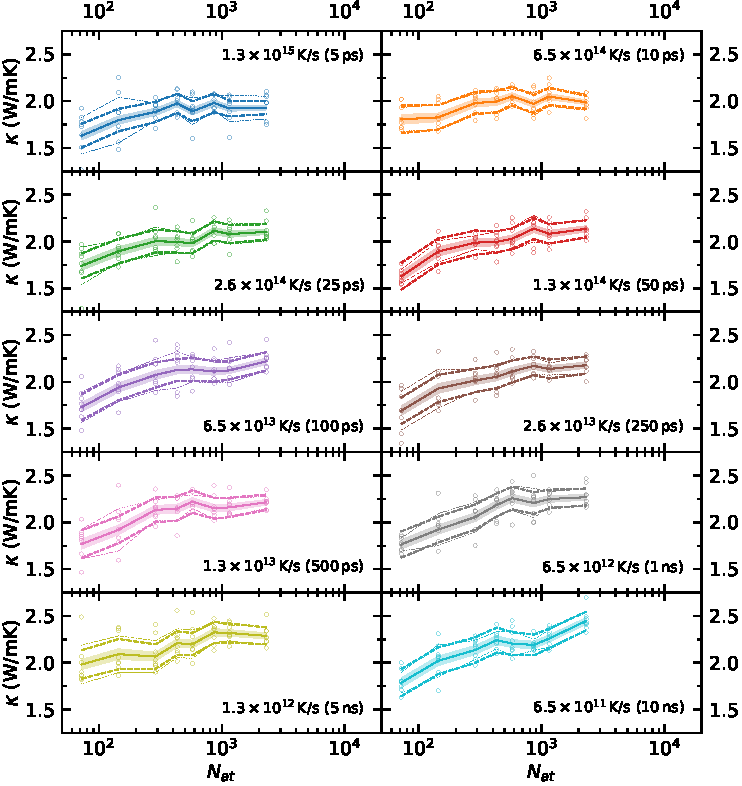
\includegraphics[width=\textwidth]{chapters/appendix/figures/Silica_NPT_kappa_NATconv.pdf}
    \caption{Thermal conductivity of a-SiO$_2$ at $500\un{K}$ obtained by a quench in the NPT ensemble at zero-pressure and with cooling rate $\gamma$. 
    The abscissa indicate the number of atoms of the system, each panel corresponds to a different quenching rate $\gamma$ (the relative quenching time $t_\mathrm{quench}$ is indicated in brackets). 
    The same symbols as Fig.~\ref{fig:results-class-kappa-vs-size} are used.
    }
    \label{fig:appendix-silica-class-npt-kappa-vs-size}
\end{figure}

\begin{figure}[!htb]
    \centering
    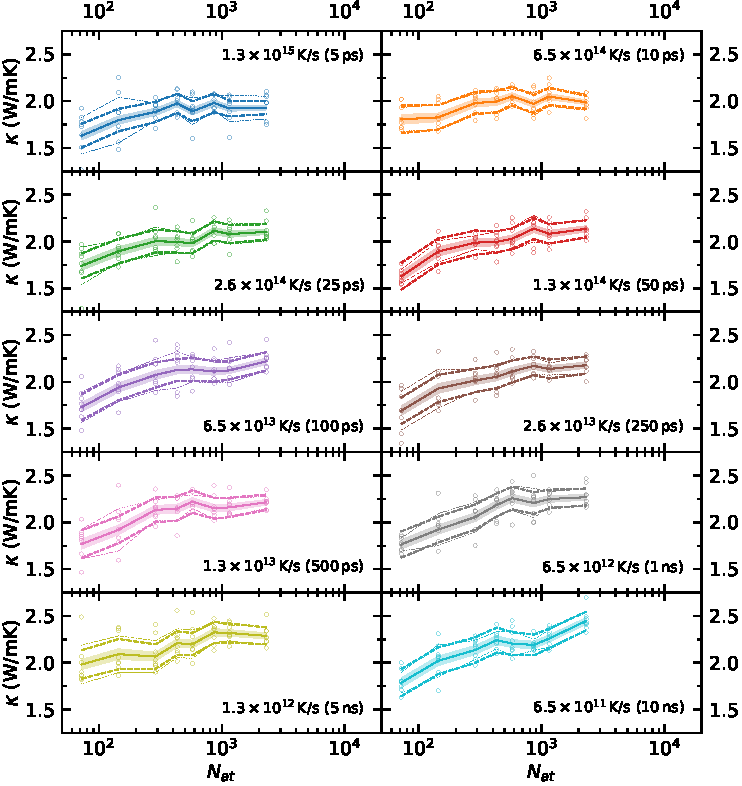
\includegraphics[width=\textwidth]{chapters/appendix/figures/Silica_NPT_kappa_NATconv.pdf}
    \caption{Thermal conductivity of a-SiO$_2$ at $500\un{K}$ obtained by a quench in the NPT ensemble at zero-pressure and with cooling rate $\gamma$. 
    Each panel corresponds to a different system size with $N_{at}$ atoms.
    The same symbols as Fig.~\ref{fig:results-class-kappa-vs-quench} are used.
    }
    \label{fig:appendix-silica-class-npt-kappa-vs-quench}
\end{figure}

\begin{figure}[!htb]
    \centering
    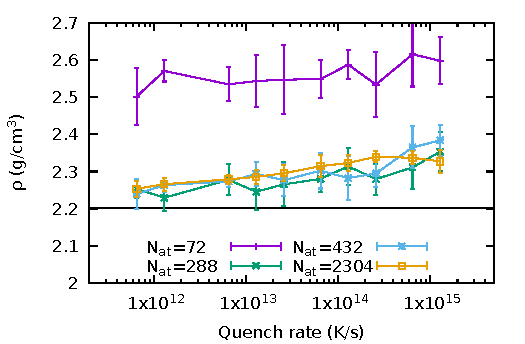
\includegraphics[width=12cm]{chapters/appendix/figures/dens_NPT_quench.pdf}
    \caption{Average density of a sample of $N_\mathrm{at}$ atoms at $500\un{K}$, obtained from a quench in the NPT ensemble at zero-pressure as a function of the quenching rate. The black line indicates the experimental value $\rho=2.202\un{g/cm^3}$. }
    \label{fig:appendix-silica-class-npt-density-vs-quench}
\end{figure}